\chapter{Conclusion}
\label{section:Conclusion}

In this thesis \ac{MRI} and \ac{MRSI} tuned to the $^2$H resonance at 3T and 7T have been used to explore some important $^2$H MR parameters such as T$_1$ relaxation times. The metabolic behaviour of $^2$H glucose has also been investigated \textit{in vivo} using \ac{DMI} at 7T. Due to this work not being performed on human scanners \textit{in vivo} at the \ac{SPMIC} previously, some of the hardware used, such as \ac{RF} coils, were in-house built and the details of designing and building of these coils have also been described here. $^2$H MRSI with $^2$H glucose is now being used to investigate metabolic diseases such as brain cancer due to the increased \ac{CNR} from metabolite concentration maps. 

\begin{figure}
    \centering
    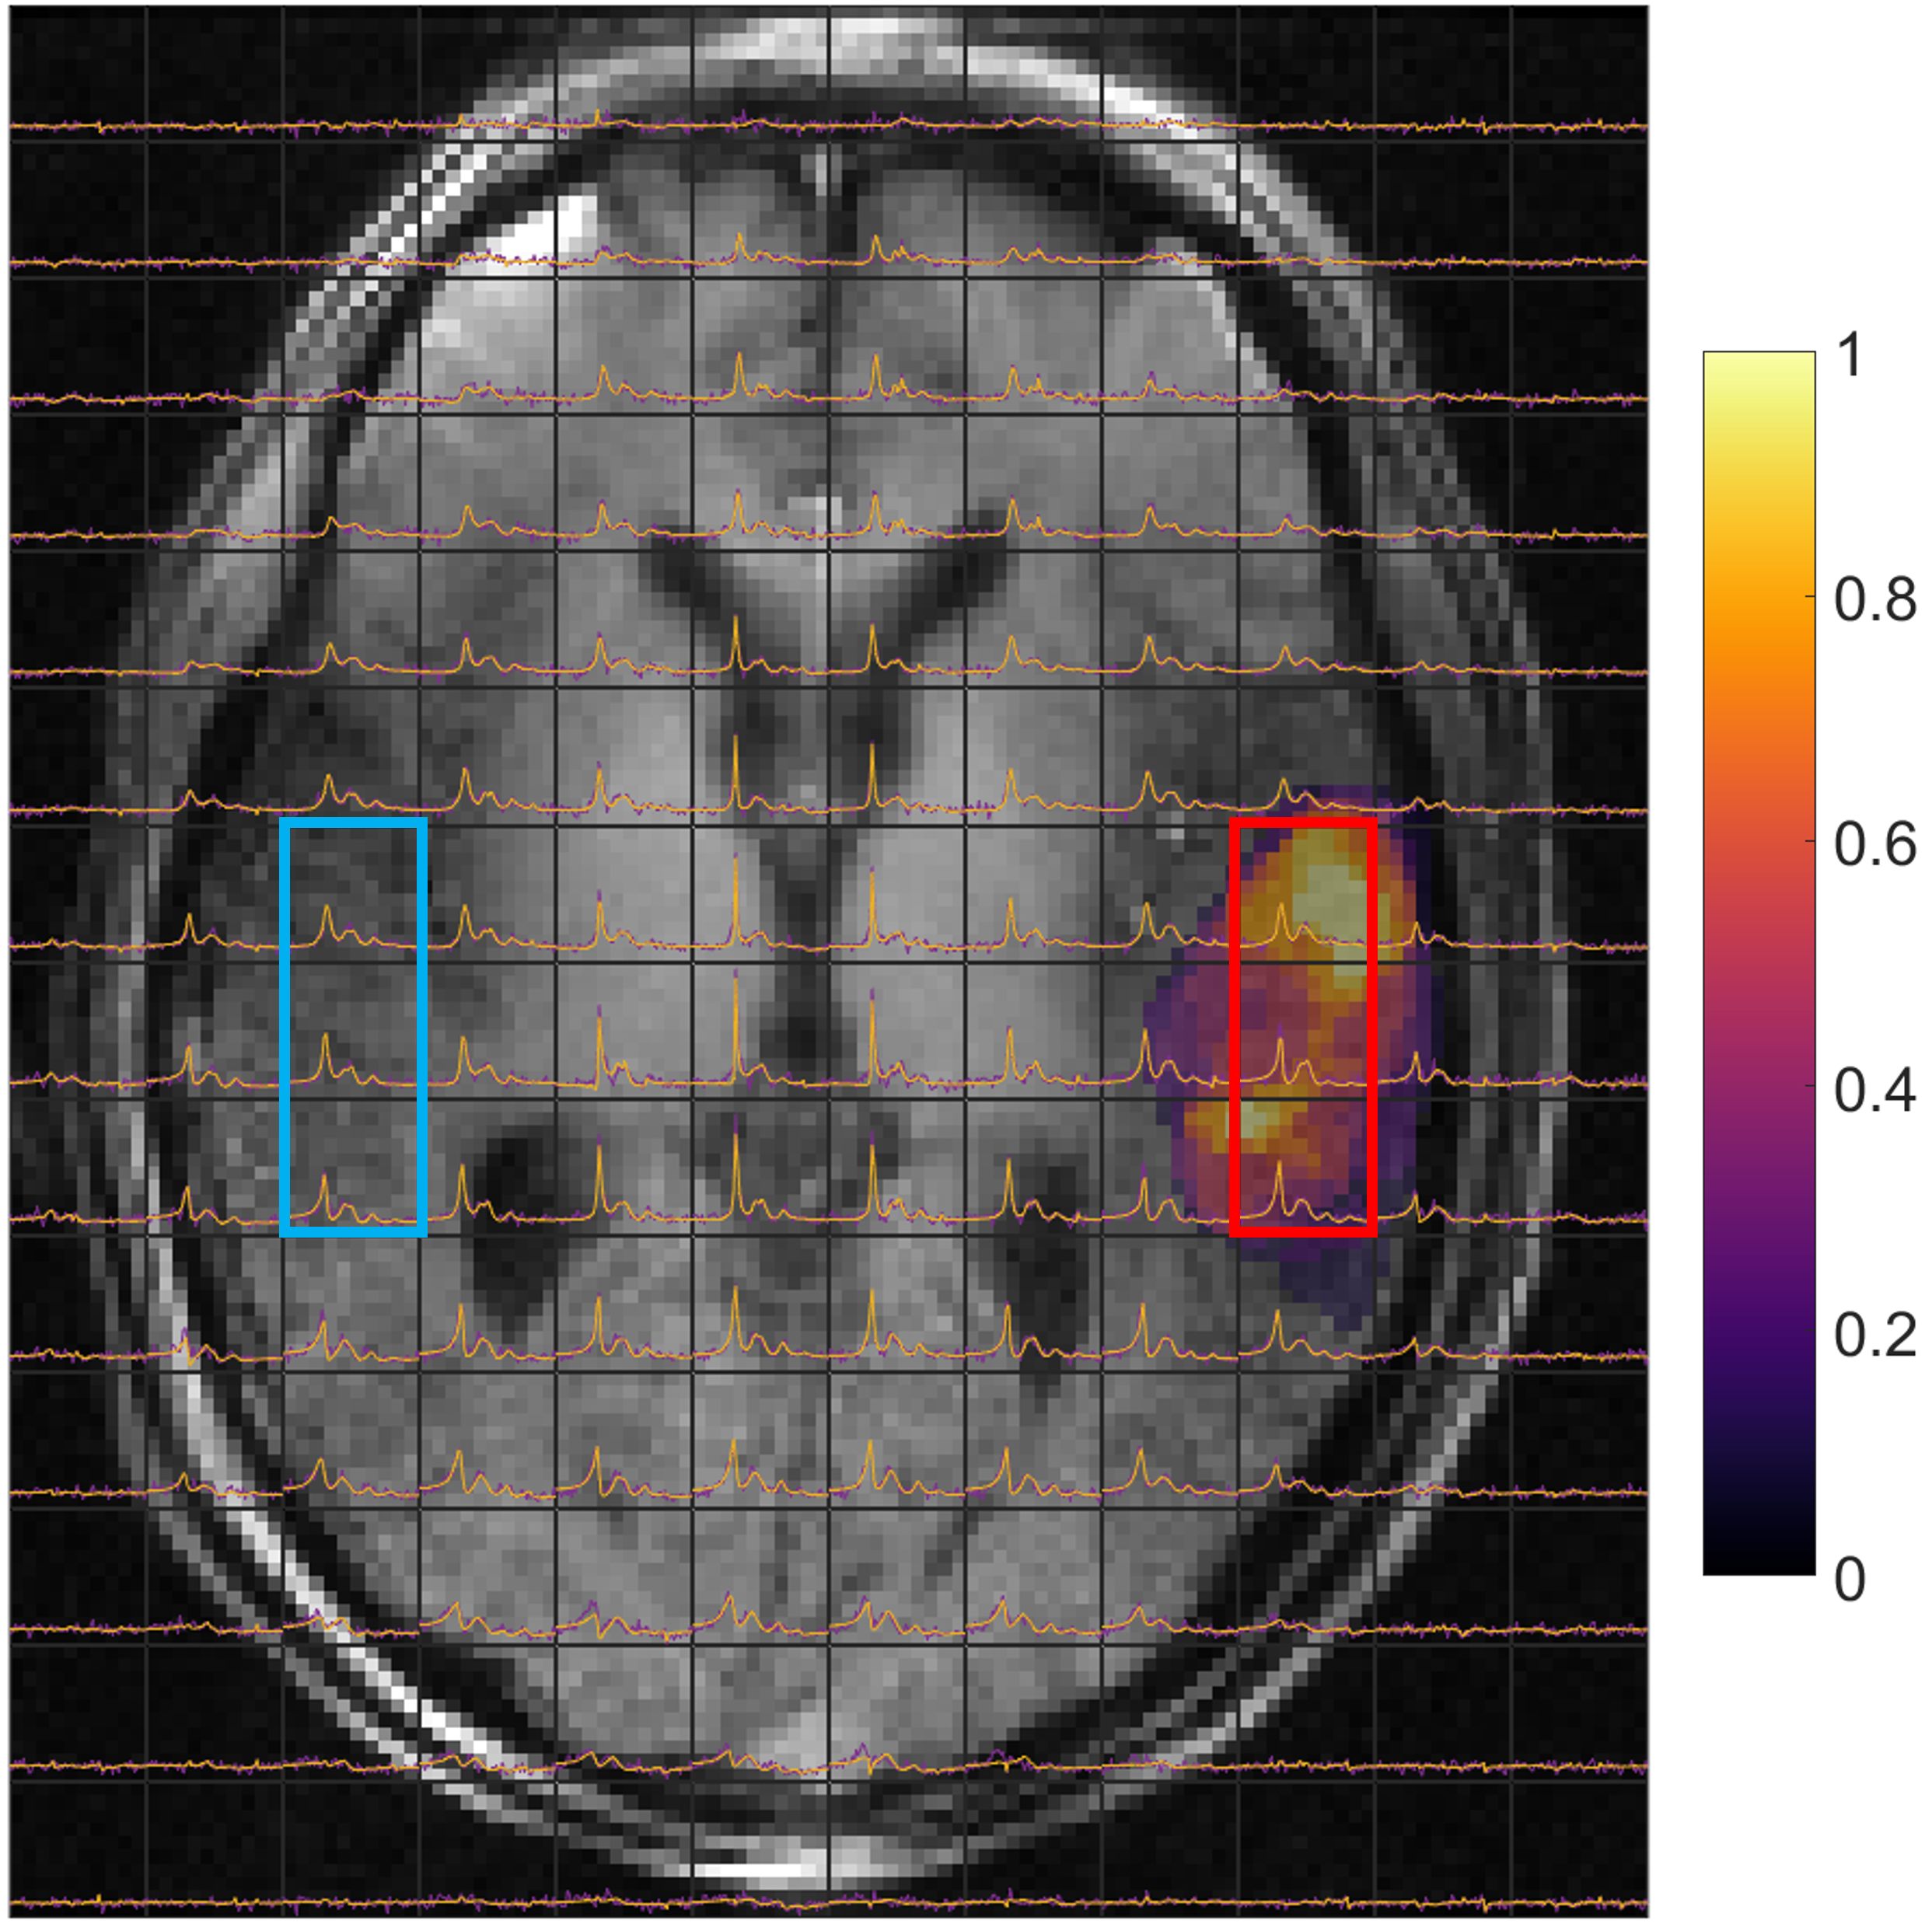
\includegraphics[width = 0.9\textwidth]{Figures/Conclusion/CSI.png}
    \caption{\textit{$^2$H CSI data acquired in $\sim$12.5 minutes (purple) along with corresponding fits (yellow). In tumour voxels (red) and contralateral voxels (blue).}}
    \label{fig:Conc:CSI}
\end{figure}

The aim of this work is to successfully lay the ground for future studies at the SPMIC to investigate brain tumours in patients using \ac{DMI} at 7T \textit{in vivo}. At the time of writing this conclusion the first DMI scan was performed in a patient with a brain tumour using ingestion of glucose-d$_7$ at 7T \textit{in vivo}, which was performed by our group at the SPMIC. In a preliminary analysis, the data has been fitted using the OXSA-AMARES toolbox \cite{Purvis2017OXSA:MATLAB} (Fig. \ref{fig:Conc:CSI}), metabolite fitting amplitudes have been obtained and tracked over time and can be seen in Fig. \ref{fig:Conc:stack} and Fig. \ref{fig:Conc:Time}. Decreased Glx was found in tumour voxels compared to contralateral voxels along with increased lactate in the three last scans. This resulted in a statistical increase in Lac/Glx in tumour voxels which is visible in Fig. \ref{fig:Conc:Box}, 0.5 $\pm$ 0.2 compared to 0.2 $\pm$ 0.2 p$<$0.05. Average metabolite maps from the post-ingestion scans are visible in Fig. \ref{fig:Conc:Maps}.

\begin{figure}[H]
    \centering
    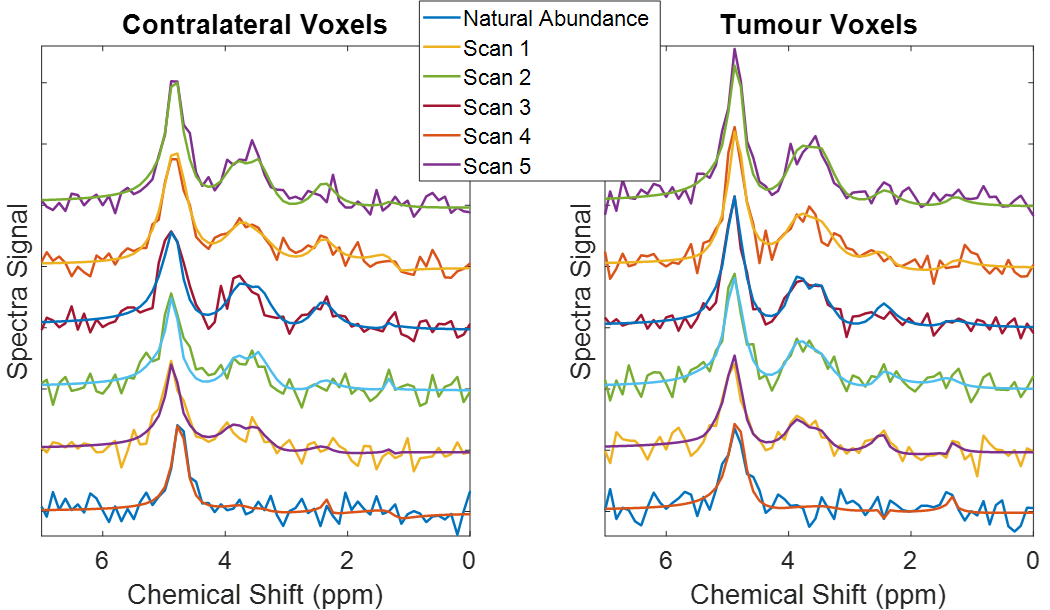
\includegraphics[width=1\linewidth]{Figures/Conclusion/Stacked.png}
    \caption{\textit{Stacked spectra along with corresponding from the contralateral voxels (left) and of the voxels that cover the tumour region (right). Each spectra is obtained by averaging the three spectra in each ROI, the fitting here is performed before the averaging.}}
    \label{fig:Conc:stack}
\end{figure}

\begin{figure}[H]
    \centering
    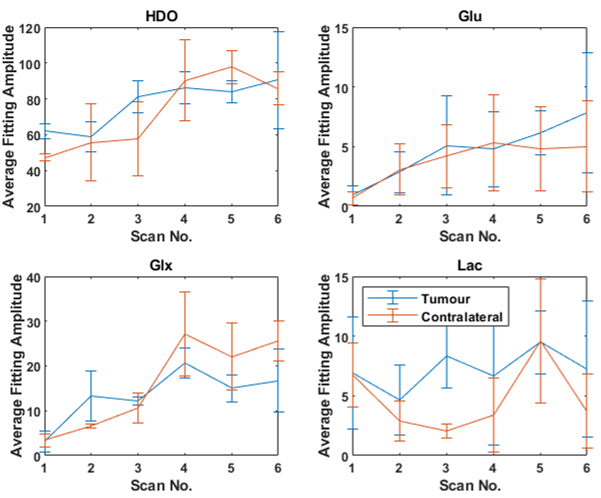
\includegraphics[width = 0.9\textwidth]{Figures/Conclusion/Time_Course.png}
    \caption{Average fitting amplitudes for each metabolite (HDO, Glucose (Glu), Glx and Lac) over the contralateral (red) voxels and the tumour (blue) voxels. For the Natural Abundance Scan (1) and the post-ingestion scans (2 to 6).}
    \label{fig:Conc:Time}
\end{figure}

\begin{figure}[H]
    \centering
    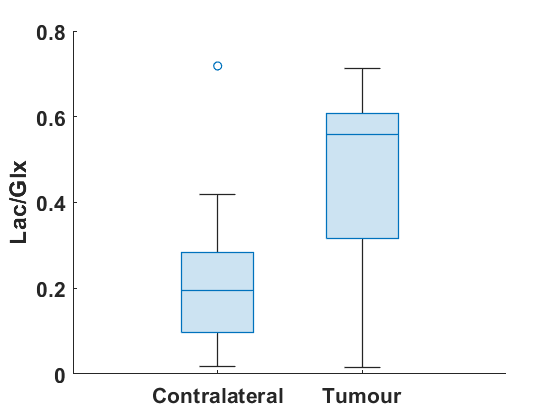
\includegraphics[width = 0.8\textwidth]{Figures/Conclusion/BarChart.png}
    \caption{Box plots for the average Lac/Glx ratios in the tumour and the contralateral voxels indicating an increase in the tumour region (p$<$0.05). For the final three post-ingestion scans where the Glx and Lac signals appear to have reached a steady state.}
    \label{fig:Conc:Box}
\end{figure}

\begin{figure}[H]
    \centering
    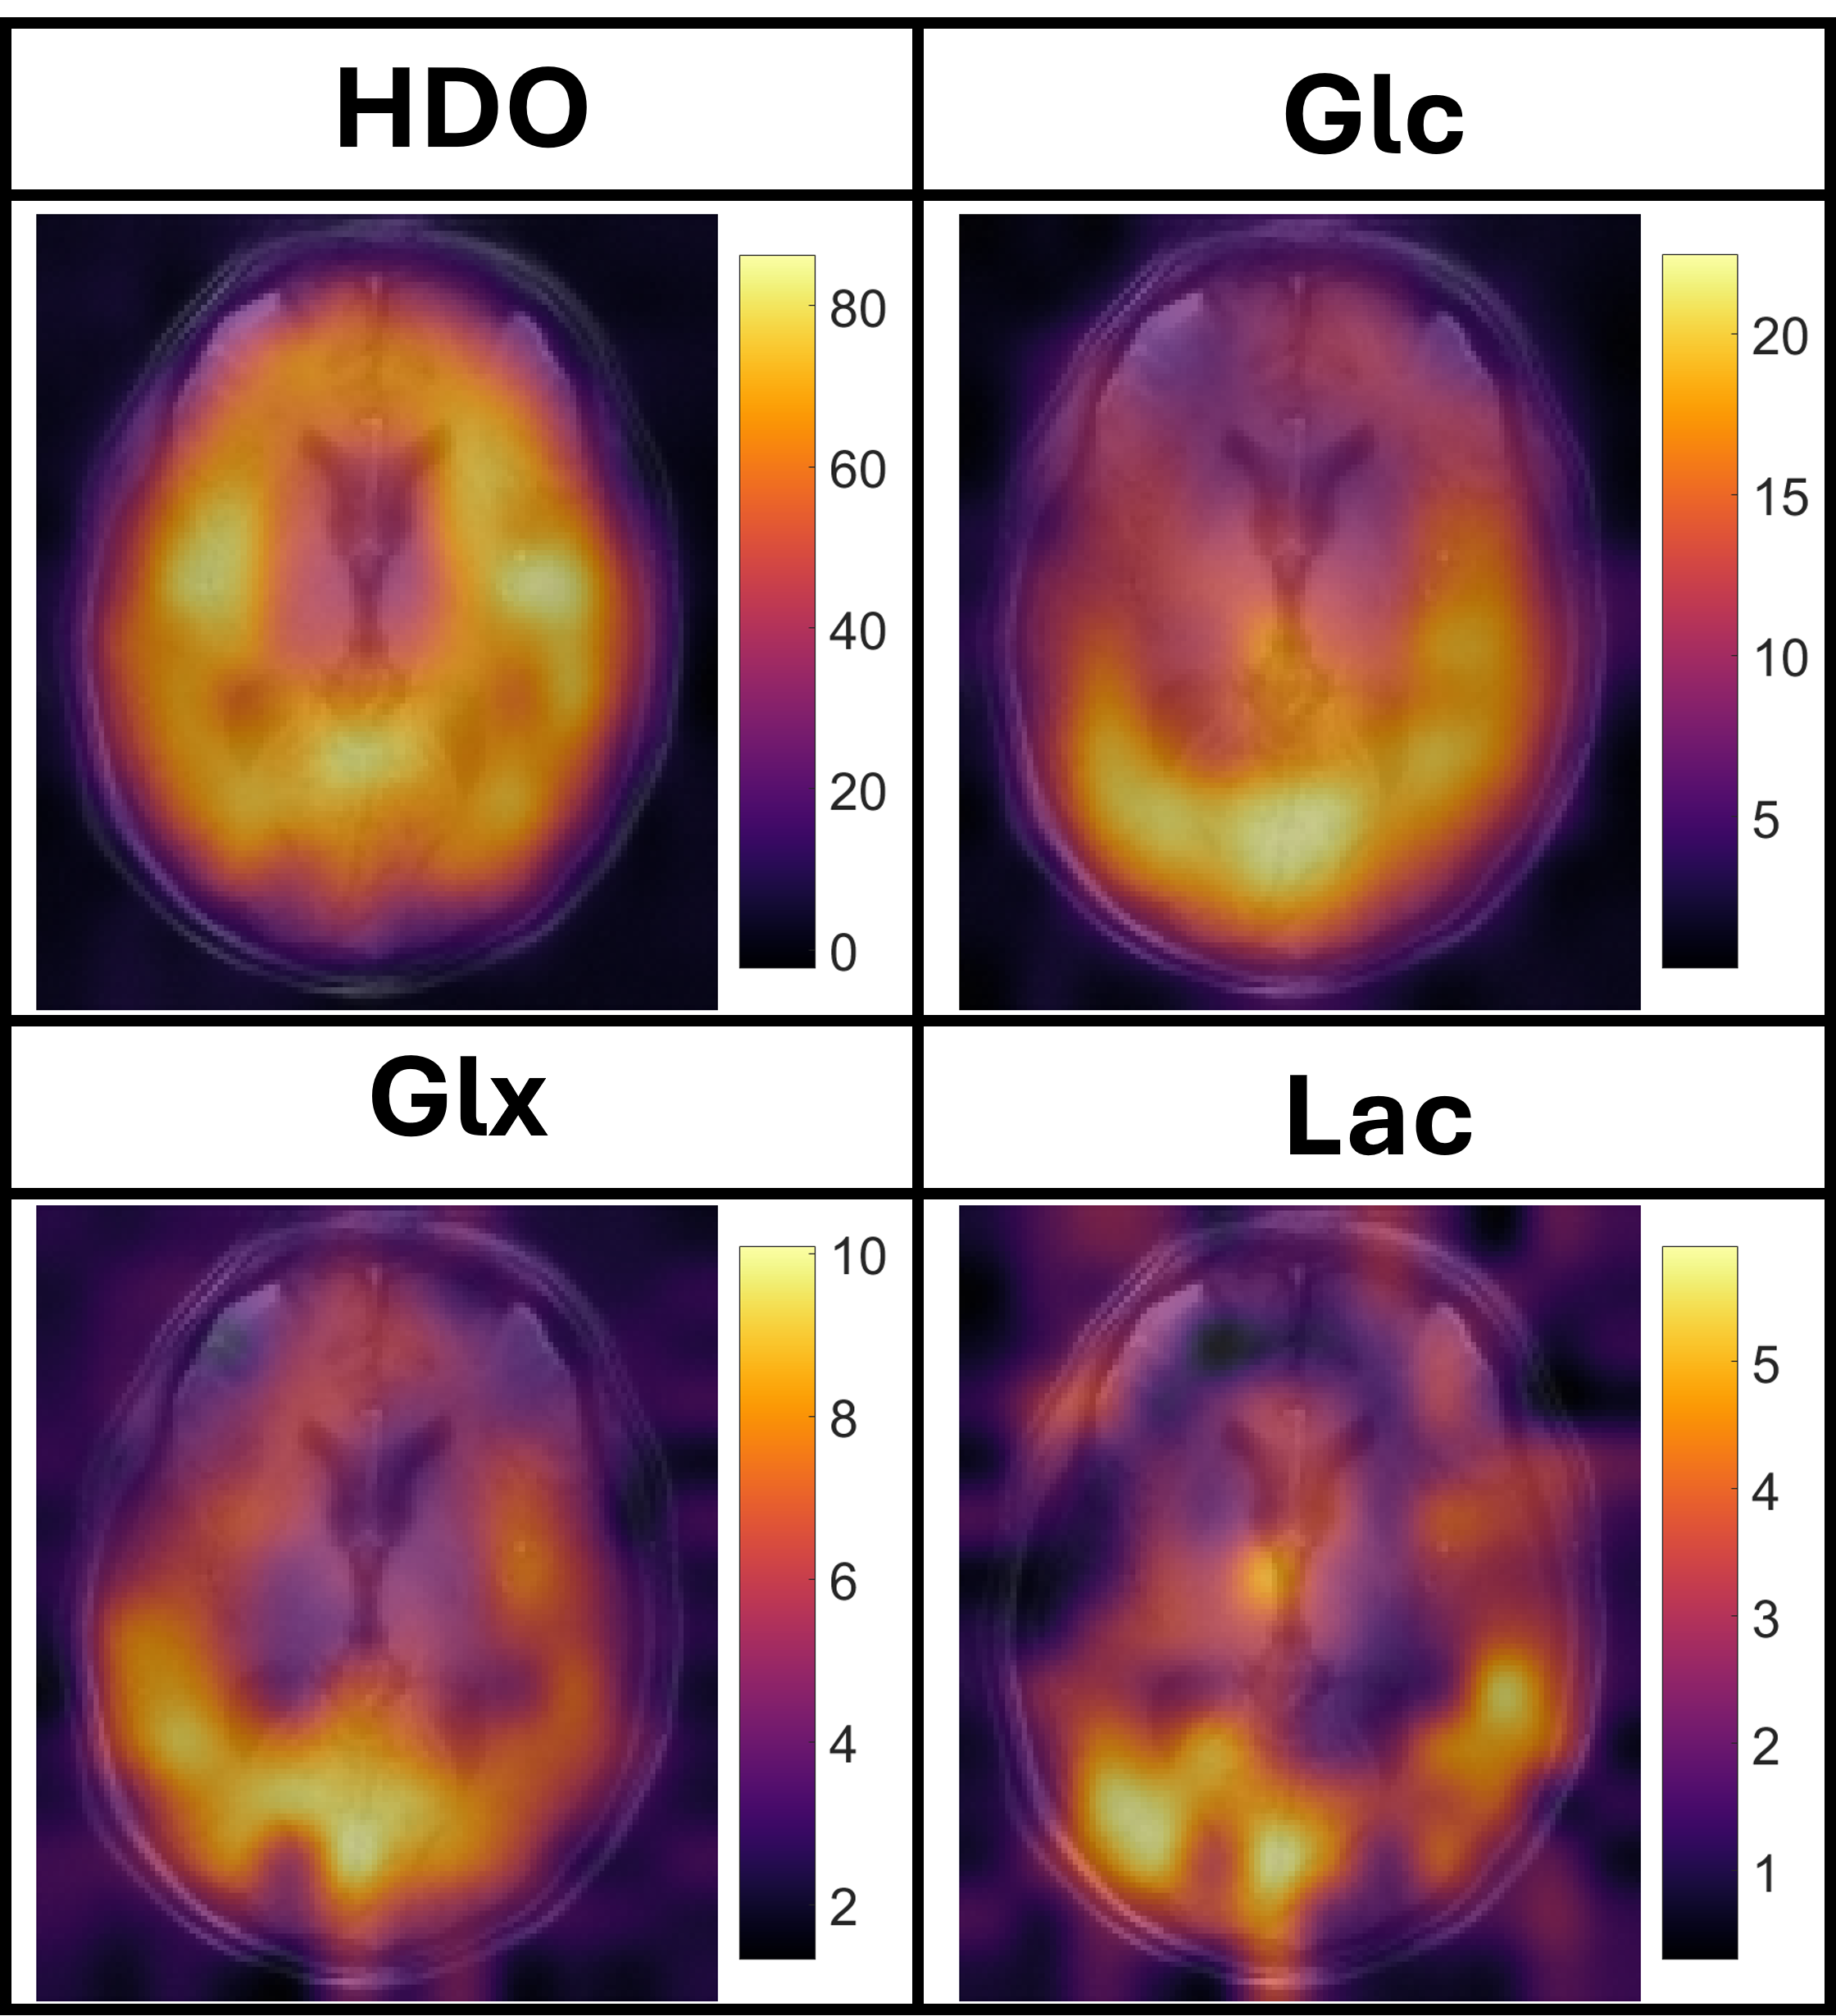
\includegraphics[width = 0.9\textwidth]{Figures/Conclusion/Maps.png}
    \caption{Average metabolite maps from the post-ingestion scans from the slice indicating the tumour.}
    \label{fig:Conc:Maps}
\end{figure}

\section{Chapter Overviews}

To obtain a complete understanding of this relatively new technique (\ac{DMI}) it is important to describe the background and history of the technique. This is done in Chapter \ref{Chap:Introduction}. The basic biology underlying metabolism and the pathways that $^2$H in a labelled compound that is ingested will take through the body are also described. The historic use of $^2$H in MR research is described in this chapter, spanning its discovery, to its use in heavy water in the 1980's in animal models and its current, most popular use in the form of $^2$H labelled glucose.

The physics that underpins the development of the experimental work in this thesis is outlined in Chapter \ref{Chap:Theory}. Initially this describes how \ac{NMR} data is obtained, going from a microscopic to a macroscopic picture. Most \ac{MRI} and \ac{MRS} research is performed by tuning to $^1$H, therefore the differences involved in tuning to the quadrupolar nucleus $^2$H are explained here. \Ac{MRSI} techniques are used throughout the work described in this thesis, so the acquisition of \ac{MRSI} data is explained in detail and the different approaches that can be used to obtain this data are explained. The mathematical approach to analysing $^2$H spectra is also detailed in this chapter, along with strategies for improving the intrinsically low \ac{SNR}. Finally the theory behind building \ac{RF} coils is described here, along with details on the electrical components.

To accurately design and optimise scanning protocols it is important to know the physical properties of the compound being scanned. One of the most important of these is the T$_1$ relaxation time, which is a key factor in selecting the \ac{TR} and the flip angle used in measurements. Measurements of the T$_1$ relaxation times of deuterated water \textit{in vivo} in \ac{CSF}, \ac{GM} and \ac{WM} at 7T are described in this chapter. Participants who were undertaking a study into cell proteomics ingested heavy water, giving rise to a hundred fold increase in the $^2$H concentration. \ac{MEGE} images with a range of \ac{TR}'s were acquired allowing joint analysis of signal variation with \ac{TE} and \ac{TR} to provide values of T$_2^*$ and T$_1$. These results were used to improve the accuracy of later concentration quantification and to improve later study/scan designs. Two of the participants were also scanned when they first began ingesting heavy water at regular intervals so that the time course of the increase in $^2$H levels could be explored, the results were found to be similar to estimates derived from simple dilution.

\begin{figure}[H]
    \centering
    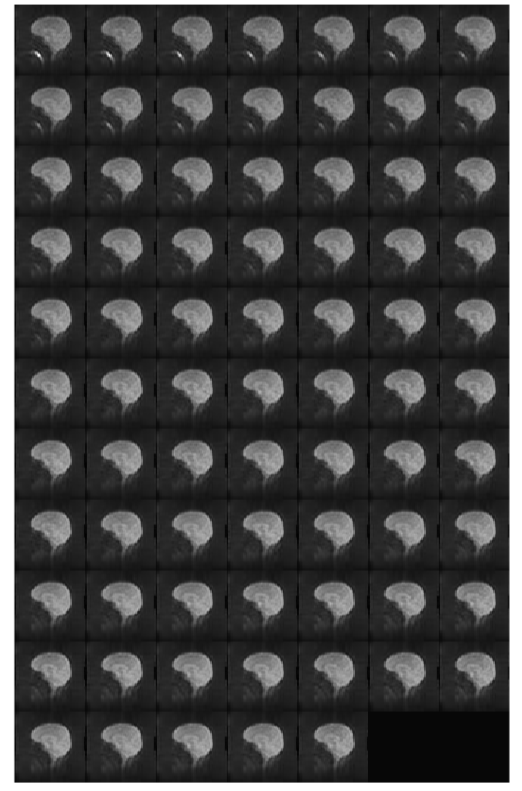
\includegraphics[width=1\textwidth]{Figures/D2O/EPI.png}
    \caption{\textit{Time-course from the five centre averaged sagittal slices of a healthy human brain in vivo, during the steady-state of D$_2$O loading, acquired using an \ac{EPI} acquisition with 75 dynamics, tuned to the $^2$H resonance at 7T.}}
    \label{fig:Conc:EPI}
\end{figure}

To demonstrate the potential of $^2$H imaging a $^2$H \ac{EPI} acquisition has been used for faster scanning during heavy water loading, allowing 75 3D image dynamics to be acquired in 48 minutes of scanning ($\sim$38 s each). A healthy human participant was scanned at 7T with a \ac{FOV}: 288 $\times$ 288 $\times$ 240 mm$^3$, voxel size: 6 $\times$ 6 $\times$ 10mm$^3$, \ac{TR}: 250 ms, TE: 13.8 ms, flip angle: 70$^\circ$, 75 dynamics, \ac{EPI} factor: 23. The participant was taking part in the studies in Chapter \ref{Chap:Lipid} and \ref{Chap:Quad} at the time of scanning and therefore followed the loading regime outlined there. The participant had completed the initial loading and was in the steady-state period. Immediately prior to scanning their 50 ml daily top-up was ingested. Traces of heavy water in the mouth and throat can be seen in the first few dynamics of Fig. \ref{fig:Conc:EPI}. The data was de-noised using a Tucker decomposition with a core matrix size of 24 $\times$ 24 $\times$ 12, afterwards the slices shown were averaged over the centre five sagittal slices. Each individual slice is shown after averaging all the temporal dynamics in Fig. \ref{fig:Conc:EPI_avg}, here no de-noising is applied.

\begin{figure}[H]
    \centering
    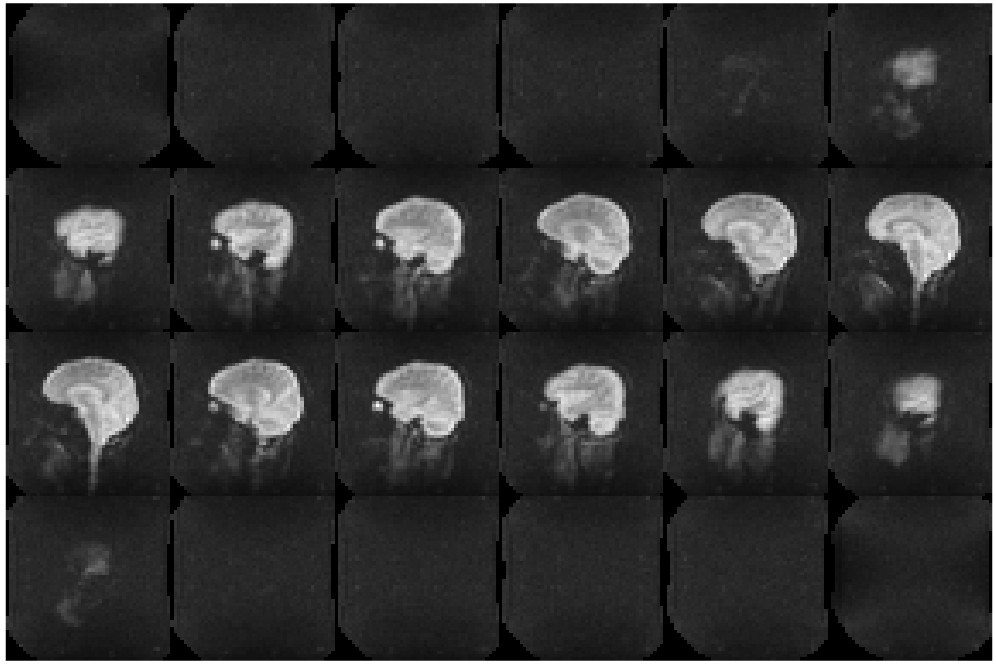
\includegraphics[width=1\textwidth]{Figures/D2O/EPI_avg.png}
    \caption{\textit{Individual sagittal slices of a healthy human brain in vivo, during the steady-state of D$_2$O loading, using an \ac{EPI} acquisition averaged over all 75 dynamics, tuned to the $^2$H resonance at 7T.}}
    \label{fig:Conc:EPI_avg}
\end{figure}

Before any work on patients can be undertaken it is important that initial measurements that involve healthy human participants are performed. This ensures that scanning protocols can be optimised for comfort and that the required scan time can be minimised. Such measurements are described in Chapter \ref{Chap:Glucose}. Healthy participants ingested glucose-d$_2$ or glucose-d$_7$ and concentration maps were subsequently obtained for \ac{HDO}, glucose, Glx and lactate. The change of signal and concentration with time was characterised and a considerable gain in \ac{SNR} when using glucose-d$_7$ versus glucose-d$_2$ for each metabolite was demonstrated.

Investigation of lipid metabolism can provide useful insights in studying metabolic diseases including diabetes, currently one of the most popular methods for such investigations involves performing invasive biopsies following heavy water ingestion. Chapter \ref{Chap:Lipid} reports the first results using $^2$H-tuned MRSI to investigate increased lipid signals following ingestion of D$_2$O. Statistically significant increases in the lipid $^2$H signal from two out of three participants in the abdomen and in 1 out of 3 in the calf were shown. This work is very new and therefore there are many ways in which a study like this can potentially be improved. These include use of water-suppression during scanning and/or post-processing. the first T$_1$ relaxation time measurements at 3T of \ac{HDO} in skeletal muscle and of deuterated lipid are also reported in this chapter.

One of the different characteristics of $^2$H compared to $^1$H is its quadrupolar moment which can cause spectral broadening/splitting in ordered tissue such as the muscle. The magnitude of quadrupolar splitting in both the forearm and the calf was quantified in different muscle groups (where possible) in Chapter \ref{Chap:Quad} and the relationship between the \ac{DQF} signal and splitting magnitude was explored. The evolution of \ac{DQF} with varying creation time ($\tau$) was also investigated. This was made possible due to the increased \ac{SNR} obtained from participants ingesting D$_2$O. This is the first time \ac{DQF} measurements have been attempted using $^2$H resonance in humans \textit{in vivo}. Accurate time-course analysis was not possible here due to potential flip angle errors and partial voluming, therefore this needs further exploration.

\section{Future Directions}

A common theme throughout the whole thesis is the use of some element of de-noising. Whilst apodisation/line-broadening has already been shown to be useful for increasing \ac{SNR} it can be problematic in causing overlap of spectral lines and can also negatively impact quantification. To avoid this issue \ac{HOSVD} is used throughout this thesis for improving \ac{SNR} and has been shown to be pivotal in improving fitting accuracy. To the author's knowledge there are currently no guidelines in the MR community on the specific level of rank-reduction that should be applied during multi-dimensional de-noising, such as with \ac{HOSVD}. Other researchers in multi-nuclear \ac{MRS} who have implemented \ac{HOSVD} have given limited justification for the rank-reduction that they have used and have generally cited previous work that has often done the same \cite{Kreis2020MeasuringMRI, vonMorze2021ComparisonT, Brender2019DynamicHyperpolarization}. It would be beneficial to the field if there was more of a focus on \ac{HOSVD} as a de-noising tool (as opposed to just a data reduction tool) and how far this method can be pushed without sacrificing spatial/temporal/spectral information. The factors that can affect \ac{HOSVD} performance also need to be further explored. For example, reshaping data matrices so that all spatial dimensions are combined into one dimension would allow the use of \ac{SVD} rather than \ac{HOSVD}. This approach would also reduce the dimensionality of time-course data making further decomposition computationally simpler.

% For example if all the spatial dimensions are combined into one dimension through a spatial trajectory then theoretically \ac{SVD} can be used. Also, if a time-course is obtained this would be the third dimension and not the fifth dimension, making the decomposition computationally simpler.

It is important to note that whilst this thesis shows how to obtain and analyse \textit{in vivo} $^2$H data, this work only sets the foundation. As has been pointed out \ac{PET}  is used for clinical studies but only provides limited metabolic information. $^2$H has the potential to provide more information. However, this first has to be shown in patient studies, as the usefulness of this technique can not truly be proven until direct comparisons are made with current clinical work. Whilst $^2$H glucose and Glx are important metabolites in the investigation of brain tumours, arguably the most important metabolite is lactate. Currently it is difficult to optimise a scan for imaging lactate as signal levels do not reach far above the noise level in scans of healthy participants. Brain tumours cause a significant increase in the lactate produced which can be detected using $^2$H \cite{Soares2009MagneticApplications}. Other metabolic diseases such as \ac{AD} and \ac{PD} also impair metabolism, which has been shown through \ac{PET} imaging\cite{Shokouhi2014ImagingTomography, Meles2017MetabolicDisease}, and therefore could potentially benefit from $^2$H scanning. It is important to optimise/reduce scan time as patients will struggle with extended periods in an MR scanner.

One of the difficulties when trying to track $^2$H incorporation into lipids after D$_2$O ingestion is the overlap of signals. When only one peak in a spectrum is visible this means standard imaging approaches can be used to map the distribution of that specific signal. If the increased \ac{HDO} signal was able to be nulled only the lipid would be visible, therefore if the same sequence was used to acquire image data more rapid acquisitions could potentially be achieved, this would improve participant/patient comfort whilst scanning or averaging can then be used to increase \ac{SNR}. However, for this to be possible almost near perfect water suppression is needed which can be difficult to achieve. In the \ac{DQF} spectra the data suffers from low \ac{SNR} as well and only has one signal present, therefore this sequence could be made into an imaging sequence which could potentially result in smaller voxels which would hopefully reduce effects from partial voluming. Therefore in the future it would be beneficial to the field if more applications of $^2$H imaging as opposed to spectroscopy, could be developed when $^2$H spectra are sparse. It's important to note this wouldn't be possible for \ac{DMI} experiments due to the multiple metabolite peaks being present.

\section{Closing Remarks}

In this thesis it has been shown that it is not only possible to obtain \textit{in vivo} $^2$H spectroscopic information in a reasonable time frame, in humans, as well as $^2$H \ac{MRI} and \ac{MRSI} at 7T. Whilst recently the use \ac{DMI} in MR research is becoming more widely popular, this thesis has shown the wide potential of uses for $^2$H and why this nucleus is becoming more popular. I hope this thesis helps push clinical strategies away from either ionising and/or invasive procedures and helps open up a pathway to more $^2$H MR research and into a place where $^2$H capabilities comes as standard in all clinical scanners.